\tikzset{every picture/.style={line width=0.75pt}} %set default line width to 0.75pt        

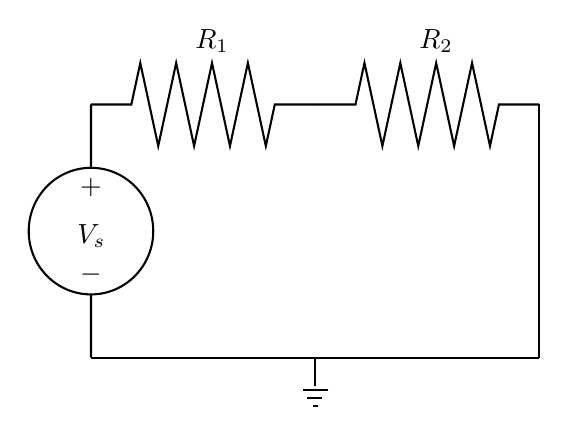
\begin{tikzpicture}[x=0.75pt,y=0.75pt,yscale=-1,xscale=1]
%uncomment if require: \path (0,300); %set diagram left start at 0, and has height of 300

%Shape: Output [id:dp694152168500714] 
\draw   (139,119.5) .. controls (155.57,119.5) and (169,133.16) .. (169,150) .. controls (169,166.84) and (155.57,180.5) .. (139,180.5) .. controls (122.43,180.5) and (109,166.84) .. (109,150) .. controls (109,133.16) and (122.43,119.5) .. (139,119.5) -- cycle (139,89) -- (139,119.5) (139,211) -- (139,180.5) ;
%Shape: Resistor [id:dp014514785173657008] 
\draw   (139,89) -- (158.44,89) -- (162.76,69) -- (171.4,109) -- (180.04,69) -- (188.68,109) -- (197.32,69) -- (205.96,109) -- (214.6,69) -- (223.24,109) -- (227.56,89) -- (247,89) ;
%Shape: Resistor [id:dp6346068220663863] 
\draw   (247,89) -- (266.44,89) -- (270.76,69) -- (279.4,109) -- (288.04,69) -- (296.68,109) -- (305.32,69) -- (313.96,109) -- (322.6,69) -- (331.24,109) -- (335.56,89) -- (355,89) ;
%Straight Lines [id:da8900340649133313] 
\draw    (139,211) -- (355,211) ;
%Straight Lines [id:da802632819816991] 
\draw    (355,89) -- (355,211) ;
%Straight Lines [id:da37478191641684244] 
\draw    (247,211) -- (247,224.42) ;
%Straight Lines [id:da6053270148706792] 
\draw    (253.42,226.42) -- (241,226.42) ;
%Straight Lines [id:da08135722826593528] 
\draw    (250.42,230.42) -- (243,230.42) ;
%Straight Lines [id:da9692312024110025] 
\draw    (248.42,234.42) -- (246,234.42) ;

% Text Node
\draw (139,122.9) node [anchor=north] [inner sep=0.75pt]    {$+$};
% Text Node
\draw (139,177.1) node [anchor=south] [inner sep=0.75pt]    {$-$};
% Text Node
\draw (139.2,152.19) node    {$V_{s}$};
% Text Node
\draw (197.32,65.6) node [anchor=south] [inner sep=0.75pt]    {$R_{1}$};
% Text Node
\draw (305.32,65.6) node [anchor=south] [inner sep=0.75pt]    {$R_{2}$};


\end{tikzpicture}
